\section{Adding images}

In this section we will look at how to add images to a \LaTeX\ document. Overleaf supports three ways to insert images:

\begin{enumerate}
    \item Use the \href{https://learn.overleaf.com/learn/Kb/How_to_insert_figures_in_Overleaf#Using_Insert_Figure_to_add_a_figure_to_your_project}{\textbf{Insert Figure} button}(
\includegraphics[height=1em]{img8-1.png}), located on the editor toolbar, to insert an image into \textbf{Visual Editor} or \textbf{Code Editor}.
    \item \href{https://www.overleaf.com/learn/how-to/How_to_paste_formatted_content_into_Overleaf%23Pasting_images_into_your_Overleaf_project}{Copy and paste an image} into \textbf{Visual Editor} or \textbf{Code Editor}.
    \item Use \textbf{Code Editor} to write LaTeX code that inserts a graphic.
\end{enumerate}

Options 1 and 2 automatically generate the LaTeX code required to insert images, but here we introduce option 3—note that you will need to \href{https://www.overleaf.com/learn/how-to/Including_images_on_Overleaf}{upload those images} to your Overleaf project. The following example demonstrates how to include a picture:

\begin{tcolorbox}
\begin{verbatim}
    \documentclass{article}
    \usepackage{graphicx} %LaTeX package to import graphics
    \graphicspath{{images/}} %configuring the graphicx package
 
    \begin{document}
    The universe is immense and it seems to be homogeneous, 
    on a large scale, everywhere we look.

    % The \includegraphcs command is 
    % provided (implemented) by the 
    % graphicx package
    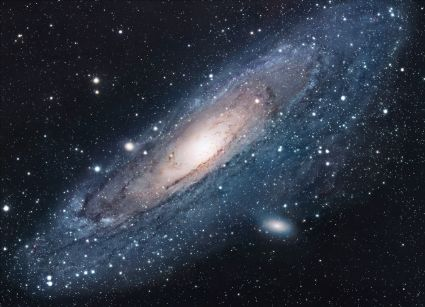
\includegraphics{universe}  
 
    There's a picture of a galaxy above.
    \end{document}
\end{verbatim}
\end{tcolorbox}

This example produces the following output:

\begin{mdframed}
\-\hspace{20pt}The universe is immense and it seems to be homogeneous, on a large scale, everywhere we look.

\-\hspace{20pt}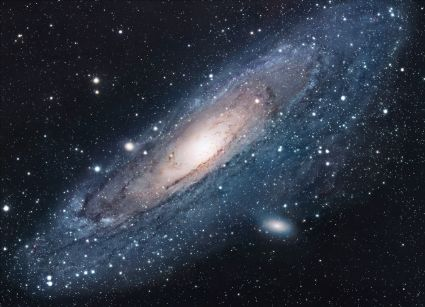
\includegraphics{universe}  
 
\-\hspace{20pt}There's a picture of a galaxy above.
\end{mdframed}

Importing graphics into a \LaTeX\ document needs an add-on package which provides the commands and features required to include external graphics files. The above example loads the graphicx package which, among many other commands, provides \\\verb|\includegraphics{...}| to import graphics and \verb|\graphicspath{...}| to advise \LaTeX \\where the graphics are located.

To use the graphicx package, include the following line in your Overleaf document preamble:

\begin{tcolorbox}
\begin{verbatim}
    \usepackage{graphicx}
\end{verbatim}
\end{tcolorbox}

In our example the command \verb|\graphicspath{{images/}}| informs \LaTeX\ that images are kept in a folder named images, which is contained in the current directory:

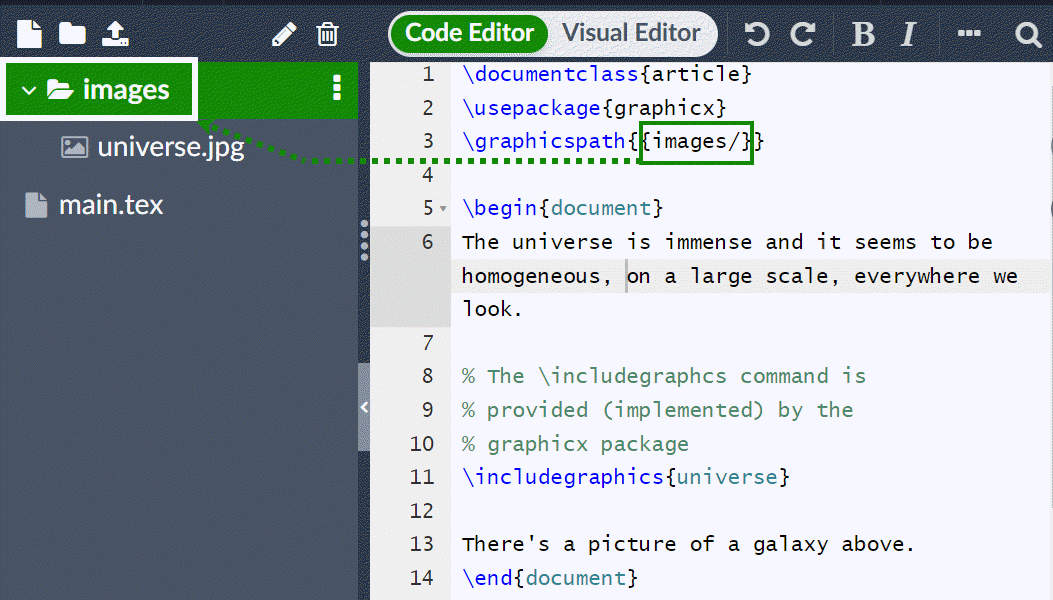
\includegraphics[width=\textwidth]{img8-2.png}

The \verb|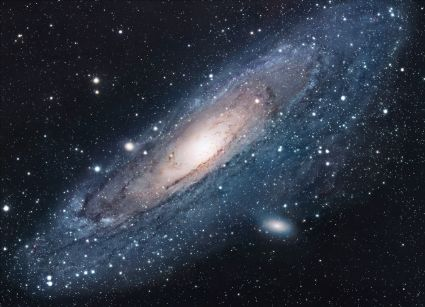
\includegraphics{universe}| command does the actual work of inserting the image in the document. Here, \verb|universe| is the name of the image file but without its extension.

\textbf{Note:}

\begin{itemize}
    \item Although the full file name, including its extension, is allowed in the \\\verb|\includegraphics| command, it’s considered best practice to omit the file extension because it will prompt \LaTeX\ to search for all the supported formats.
    \item Generally, the graphic’s file name should not contain white spaces or multiple dots; it is also recommended to use lowercase letters for the file extension when uploading image files to Overleaf.
\end{itemize}

More information on \LaTeX\ packages can be found at the end of this tutorial in the section \href{https://www.overleaf.com/learn/latex/Learn_LaTeX_in_30_minutes#Finding_and_using_LaTeX_packages}{Finding and using LaTeX packages}.